\documentclass{beamer}
\usetheme{CambridgeUS}
\usepackage {preamble}
\begin{document}

\author{Потапкина Маргарита, 251 группа \\ Научный руководитель: доцент, к.ф"=м.н. Батраева Инна Александровна}
\title{Аллокаторы памяти в языке C++}
\institute{
Саратовский государственный университет имени Н. Г. Чернышевского

Факультет компьютерных наук и информационных технологий

Кафедра математической кибернетики и компьютерных наук
}
\date{29.06.2026}
\maketitle

\setminted{obeytabs=true, tabsize=4, autogobble=true}

\begin{frame}[plain]
\frametitle{Цели и задачи работы}
\justifying 
\textbf{Цель работы} "--- проведение сравнительного анализа различных алгоритмов аллокации памяти и реализация собственного аллокатора. 

\textbf{Задачи работы}:
\begin{itemize}
	\item изучение реализации стандартного аллокатора в языке C++;
	\item проведение обзора и классификации существующих алгоритмов аллокации памяти и реализация некоторых из этих алгоритмов на языке C++;
	\item создание и реализация собственного алгоритма аллокации памяти на базе существующих с применением некоторых оптимизаций;
	\item выполнение сравнительного анализа существующих алгоритмов, а также собственного алгоритма, с целью сравнения их быстродействия.
\end{itemize}
\end{frame}

\begin{frame}[plain]
\frametitle{Что такое аллокатор?}
\justifying
\begin{block}{}
Аллокаторы (\textit{allocator} "--- распределитель памяти) "--- абстракция, которая используется с целью изоляции разработчика алгоритмов и контейнеров, нуждающихся в выделении памяти, от низкоуровневых деталей физической организации памяти. 
\end{block}

\textbf{Стандартный	аллокатор} \texttt{std::allocator} "--- использует операторы \texttt{new} и \texttt{delete}, которые обращаются к функциям выделения памяти операционной системы.

\textbf{Пользовательские аллокаторы} "--- реализуют альтернативные схемы работы с памятью, применяются в:

\begin{itemize}
	\item разработке игр;
	\item работе с БД;
	\item защищённых и встраиваемых ОС.
\end{itemize}
\end{frame}

\begin{frame}[plain]
\frametitle{Стандартный VS пользовательский аллокатор}
\justifying
\begin{figure}[H]
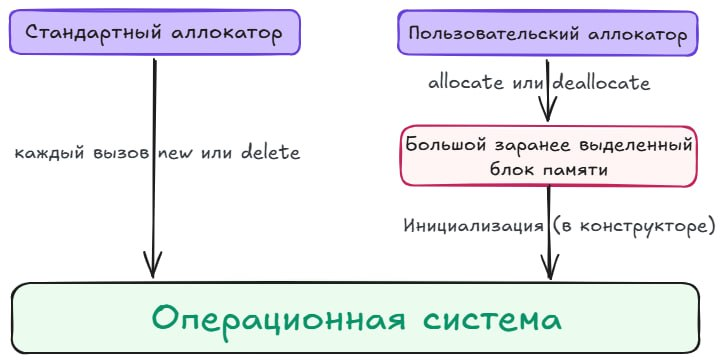
\includegraphics[scale=0.55]{difference.png}
\centering
\end{figure}
Постоянное обращение к операционной системе приводит к снижению производительности, а также может вызвать фрагментацию памяти или её утечки (в случае, если память не освобождается своевременно). Напротив, схема пользовательского аллокатора оптимизирует работу с памятью.
\end{frame}

\begin{frame}[plain]
\frametitle{Виды пользовательских аллокаторов}
\justifying
\begin{figure}[H]
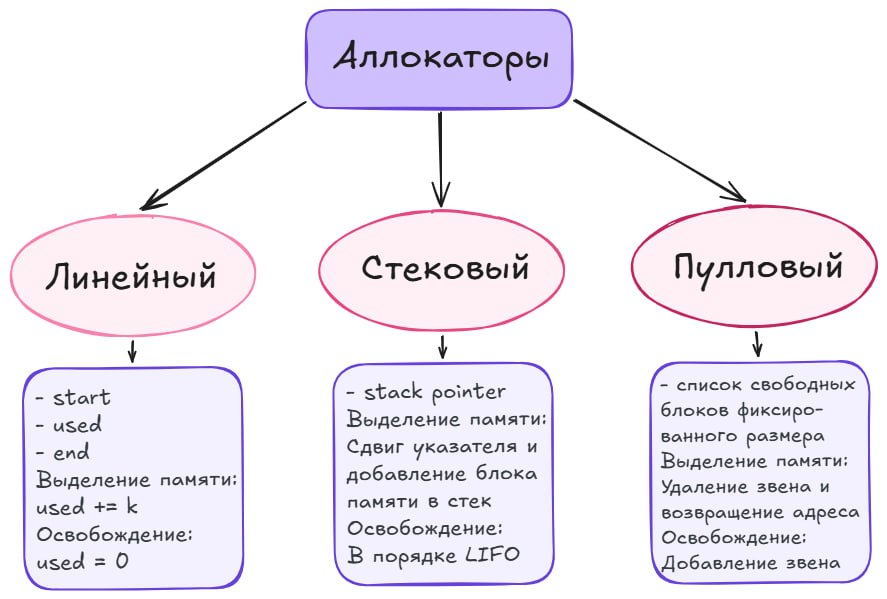
\includegraphics[scale=0.48]{allocators.png}
\centering
\end{figure}
\end{frame}

\begin{frame}[plain,fragile]
\frametitle{Реализация существующих аллокаторов}
\justifying
\begin{columns}[T]
\begin{column}{0.6\textwidth}
\begin{itemize}
	\item полиморфные методы \texttt{allocate}, \texttt{deallocate}, \texttt{reset};
	\item разработка классов для линейного, пуллового и стекового аллокатора;
	\item написание обёртки над стандартным аллокатором;
	\item разработка тестовой функции, которая:
	\begin{enumerate}
		\item создаёт массив из $n$ элементов, являющихся указателями на \texttt{int};
		\item присваивает каждому из элементов некоторое тривиально вычисляемое значение;
		\item производит очистку памяти в определённом порядке:
		\begin{itemize}
		\item для стекового "--- в обратном выделению;
		\item для пуллового "--- в произвольном;
		\item для линейного "--- метод \texttt{reset}.
		\end{itemize}
	\end{enumerate}
\end{itemize}
\end{column}

\begin{column}{0.4\textwidth}
\scriptsize
\begin{minted}{cpp}
struct LinearAllocator {
	void* start;
	int end;
	int used;
	LinearAllocator(int size) { 
		start = malloc(size);
		end = size;
		used = 0;
	}
	~LinearAllocator() {
		free(start);
	}
	void* allocate(int k) {
    	if (used + k > end) 
			return nullptr;
		void* ptr = ((char*)start
					+ used);
    	used += k;
    	return ptr;
	}
	void deallocate(void* ptr) {}
  	void reset() {
    	used = 0;
  	}
};
\end{minted}
\normalsize
\end{column}
\end{columns}
\end{frame}

\begin{frame}[plain]
\frametitle{Реализация тестовой функции}
\justifying
\begin{block}{}
\inputminted{cpp}{test_function.cpp}
\end{block}
При тестировании было выбрано $n = 100000$. Для замера точного времени выполнения использовалась функция \texttt{chrono::high\_resolution\_clock::now()}.
\end{frame}

\begin{frame}[plain]
\frametitle{Сравнение скорости работы аллокаторов}
\justifying
\input{../diagram_1.tex}
\end{frame}

\begin{frame}[plain]
\frametitle{Разработка собственного аллокатора}
\justifying
\begin{alertblock}{Постановка задачи}
Хранение структур с несколькими полями на примере пар чисел.
\end{alertblock}

\begin{block}{Варианты решения}
\begin{itemize}
\item хранение данных по строкам "--- выделение памяти сначала под первый элемент пары, затем под второй; классический подход.
\begin{figure}[H]
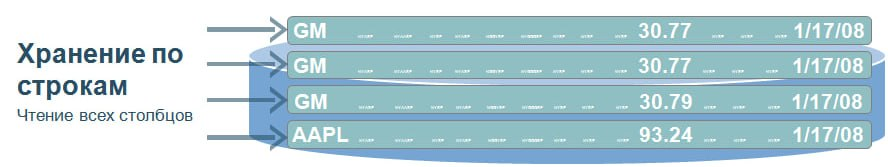
\includegraphics[scale=0.4]{rows.png}
\centering
\end{figure}
\item хранение данных по столбцам "--- выделение памяти отдельно по каждому полю; подход, основанный на \textit{колоночных базах данных}.
\begin{figure}[H]
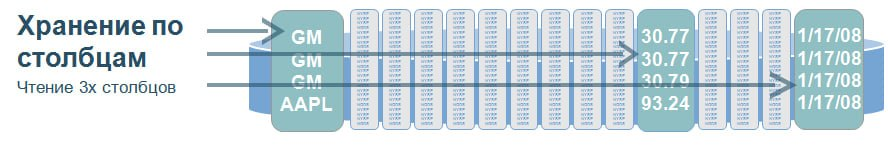
\includegraphics[scale=0.4]{columns.png}
\centering
\end{figure}
\end{itemize}
\end{block}
\end{frame}

\begin{frame}[plain,fragile]
\frametitle{Колоночный аллокатор}
\justifying
\begin{columns}[c]
\begin{column}{0.5\textwidth}
В основе <<колоночного аллокатора>> лежит пулловый аллокатор, однако в качестве полей он содержит два списка свободных блоков и два пула памяти: под координаты $x$ и $y$.

Может обеспечить ускорение при:
\begin{itemize}
\item освобождении памяти по столбцам;
\item итерации по одному из полей структуры;
\item чтении, сортировке или суммировании значений только по одной из координат.
\end{itemize}
\end{column}

\begin{column}{0.5\textwidth}
\scriptsize
\begin{minted}{cpp}
struct ColumnAllocator {
	list* free_x;
	list* free_y;
	void* pool_x;
	void* pool_y;
	int block_count;
	int block_size;
	ColumnAllocator(int object_size,
					int n) {}
	~ColumnAllocator() {}
	int* allocate_x(int k) {
		if (! free_x) return nullptr;
		list* block_x = free_x;
		free_x = free_x->next;
		return (int*)block_x;
	}
	void deallocate_x(int* ptr) {
		if (! ptr) return;
		if (((char*)ptr - (char*)pool_x)
			% block_size != 0) return;
		list* block_x = (list*)ptr;
		block_x->next = free_x;
		free_x = block_x;
	}
}
\end{minted}
\normalsize
\end{column}
\end{columns}
\end{frame}

\begin{frame}[plain]
\frametitle{Сравнение собственного аллокатора с существующими}
\justifying
\pgfplotsset{compat=newest}

\begin{figure}[H]
\begin{tikzpicture}
	\begin{axis}[
	ybar,
	bar width=18pt,
	width=\textwidth,
	height=7.5cm,
	ymin=0,
	ylabel={Среднее время},
		legend style={at={(0.5, 0.7)},
					  anchor=south},
	symbolic x coords={
		Пулловый,
		Колоночный,
		Стандартный},
	xtick=data,
	nodes near coords={
    	\pgfmathfloattofixed{\pgfplotspointmeta}
    	\pgfmathprintnumber[fixed,precision=4]{\pgfmathresult}
	},
	nodes near coords align={vertical},
	every node near coord/.append style={font=\small},
	enlarge x limits=0.2,
	grid=both,
	]
	\addplot coordinates {
	(Пулловый,0.078153)
	(Колоночный,0.109519)
	(Стандартный,0.281971)
	};
	\addplot+[bar shift=18pt] coordinates {
	(Пулловый,0.119514)
	(Колоночный,0.074305)
	(Стандартный,0.358355)
	};
	\legend{Освобождение по строкам, Освобождение по столбцам}
	\end{axis}
\end{tikzpicture}
\caption{Сравнение скорости работы аллокаторов на парах чисел}
\label{fig:pair_results}
\end{figure}

\end{frame}

\begin{frame}[plain]
\frametitle{Выводы}
\justifying
\begin{itemize}
\item Линейный, стековый и пулловый аллокатор являются достаточно простыми в реализации, в то же время их выигрыш в производительности по сравнению со стандартным аллокатором огромен: было достигнуто ускорение в $3,25$ (для пуллового) -- $19,05$ (для линейного и стекового) раз.
\item Необходимо избегать бездумных вызовов \texttt{new} и \texttt{delete}, поскольку они сильно замедляют работу программы.
\item Далеко не у каждого разработчика хотя бы раз в жизни возникает необходимость реализовать собственный аллокатор, и для большинства нужд вполне подходящим оказывается стандартный аллокатор языка C++.
\item Изучение различных алгоритмов аллокации позволяет выявить причины замедлений в программе и при необходимости заменить стандартный алгоритм аллокации некоторым пользовательским вариантом.
\end{itemize}
\end{frame}

\end{document}
